\chapter{Artículos publicados y enviados en orden cronológico}
\begin{figure}[H]
	\centering
	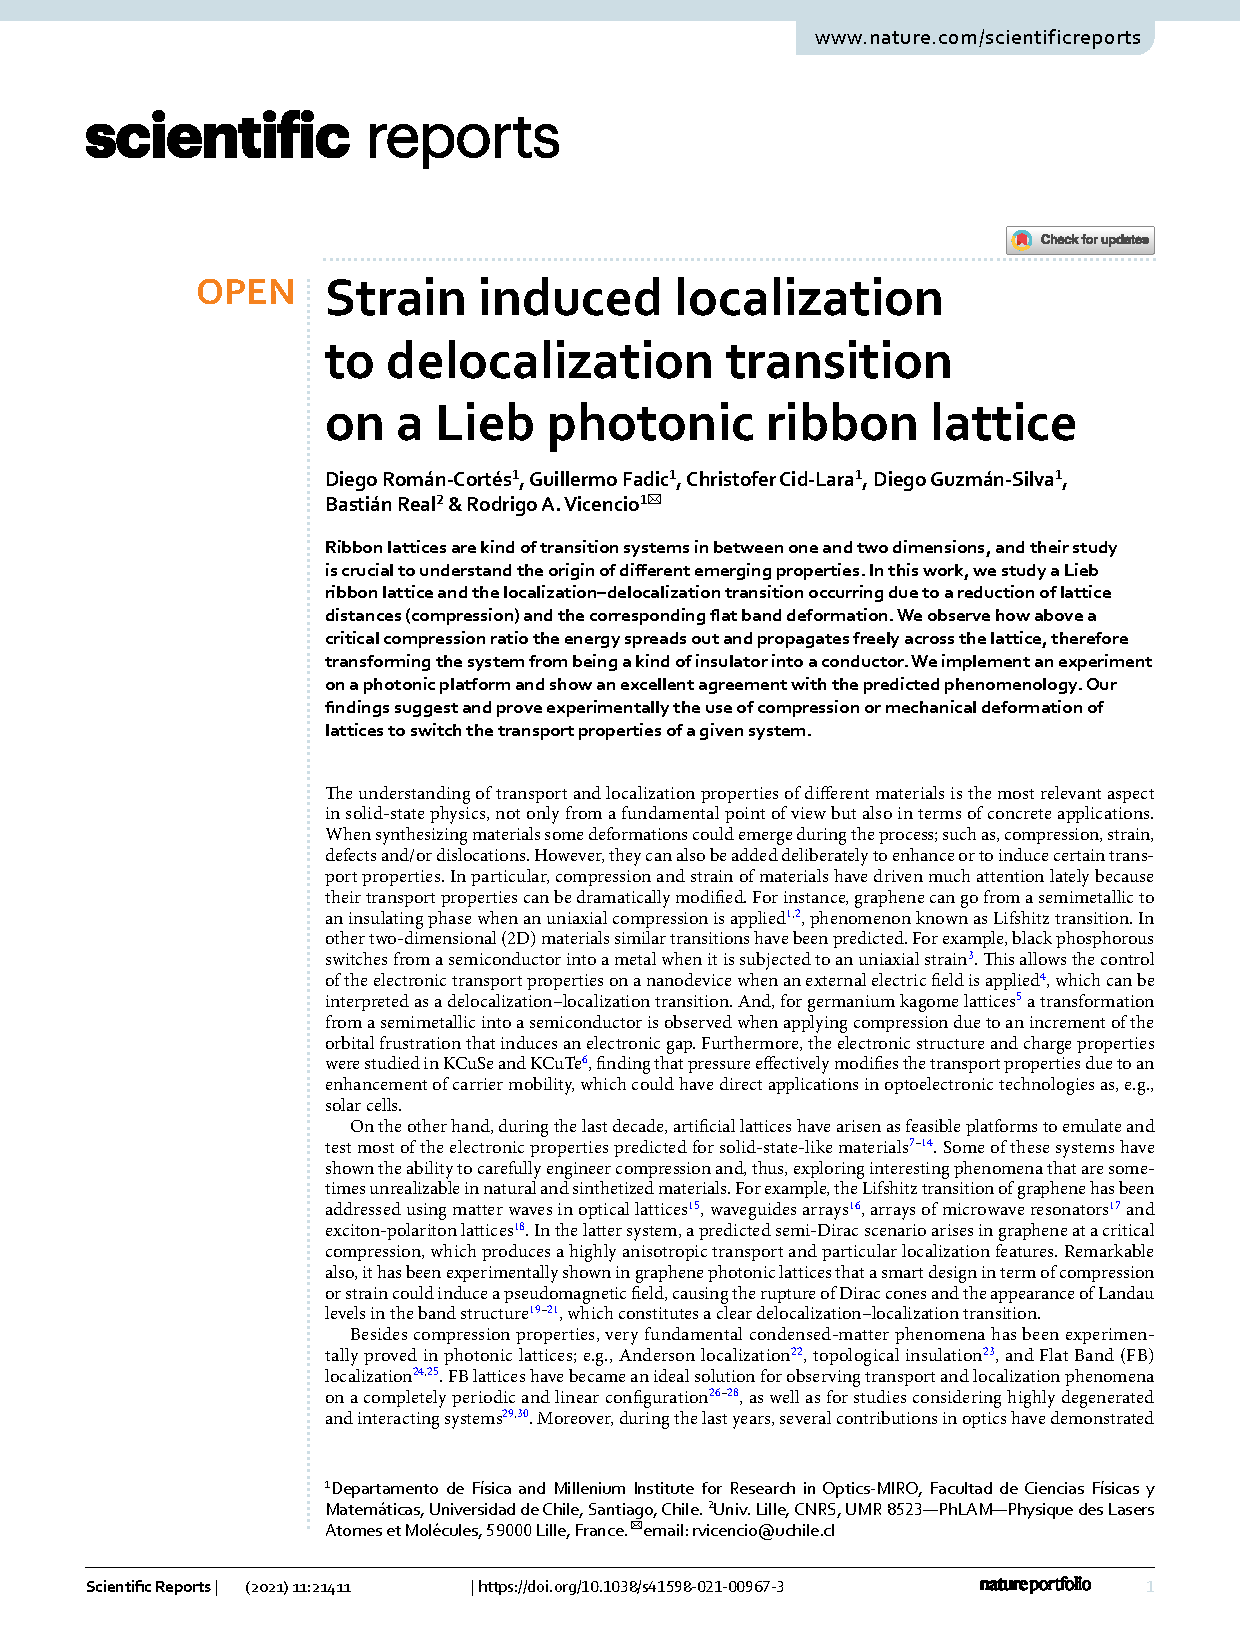
\includegraphics[page=1, width=0.9\linewidth]{media/strainlieb.pdf}
\end{figure}
\newpage
\begin{figure}[H]
	\centering
	\includegraphics[page=1, width=\linewidth]{media/molpap.pdf}
\end{figure}
\newpage
\begin{figure}[H]
	\centering
	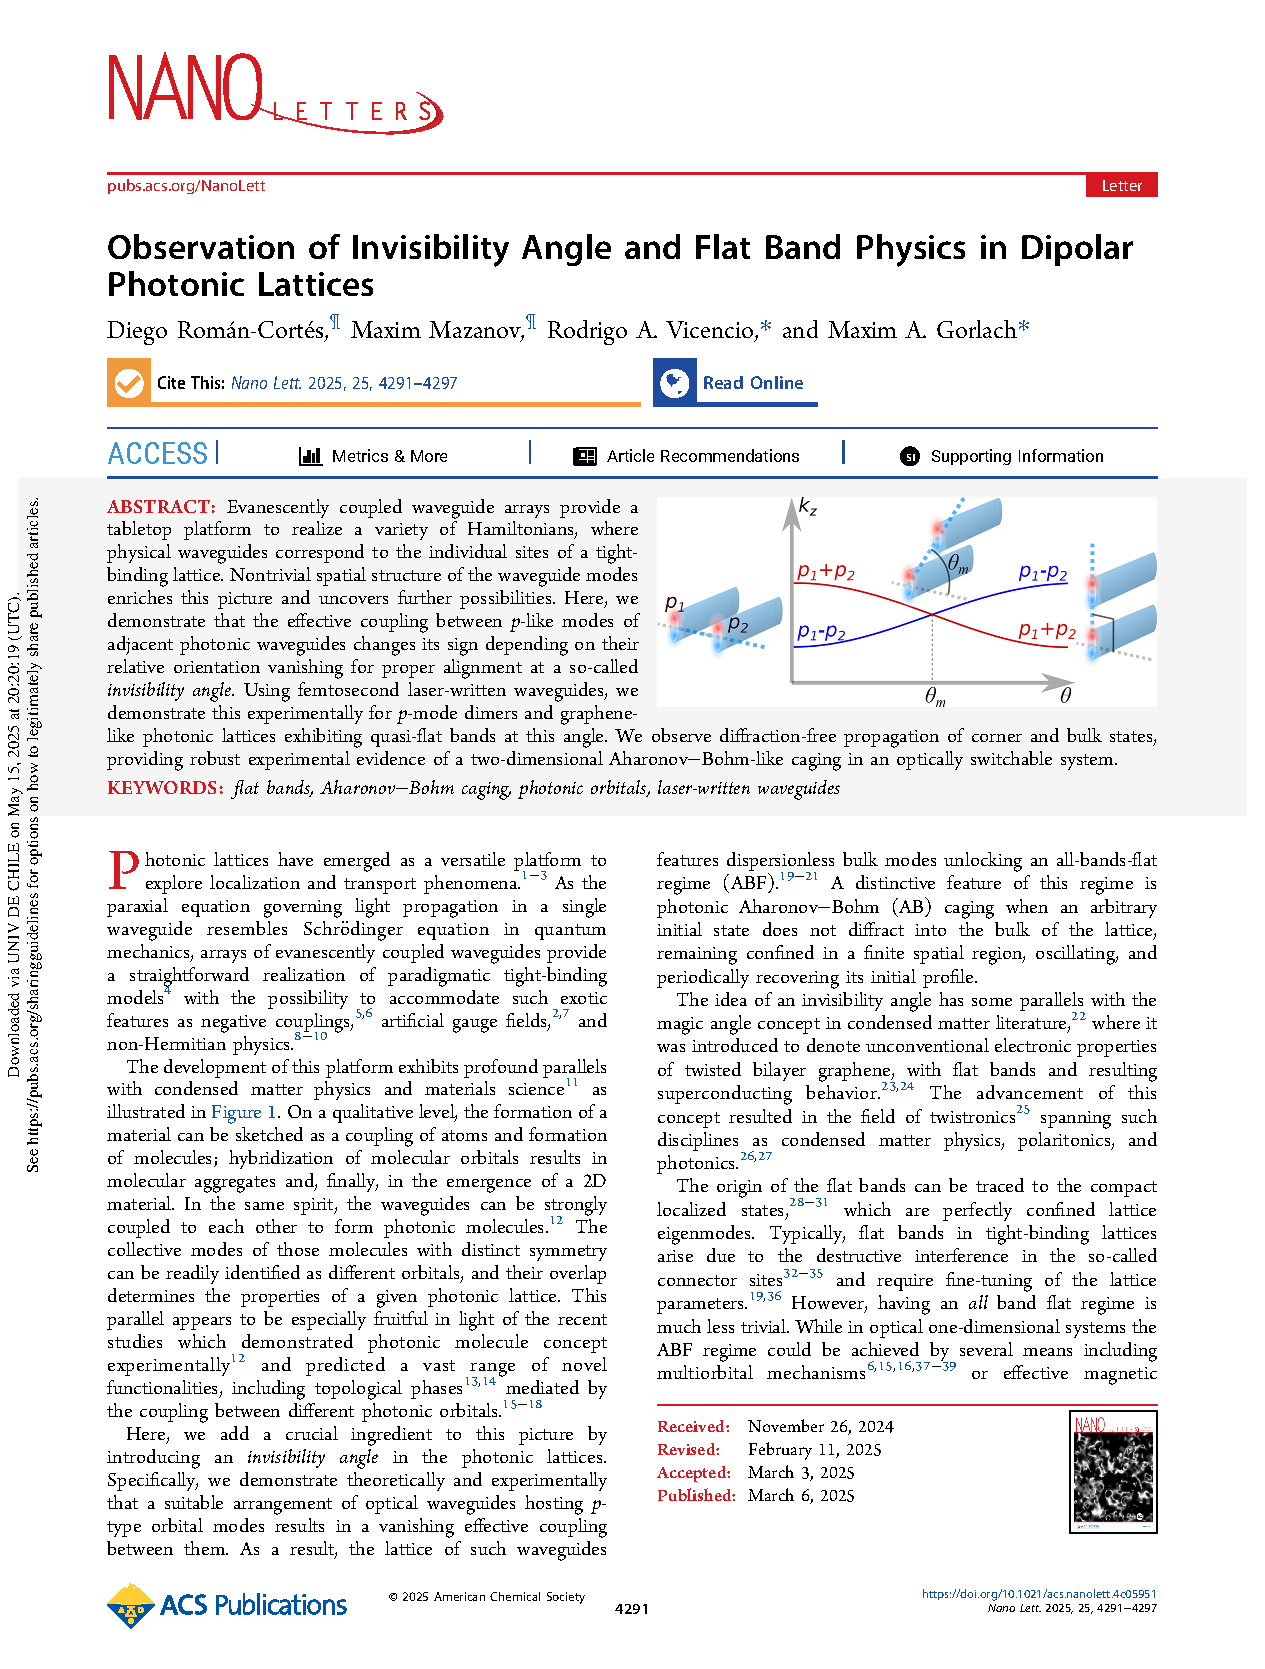
\includegraphics[page=1, width=\linewidth]{media/dipolepap.pdf}
\end{figure}
\newpage
\begin{figure}[H]
	\centering
	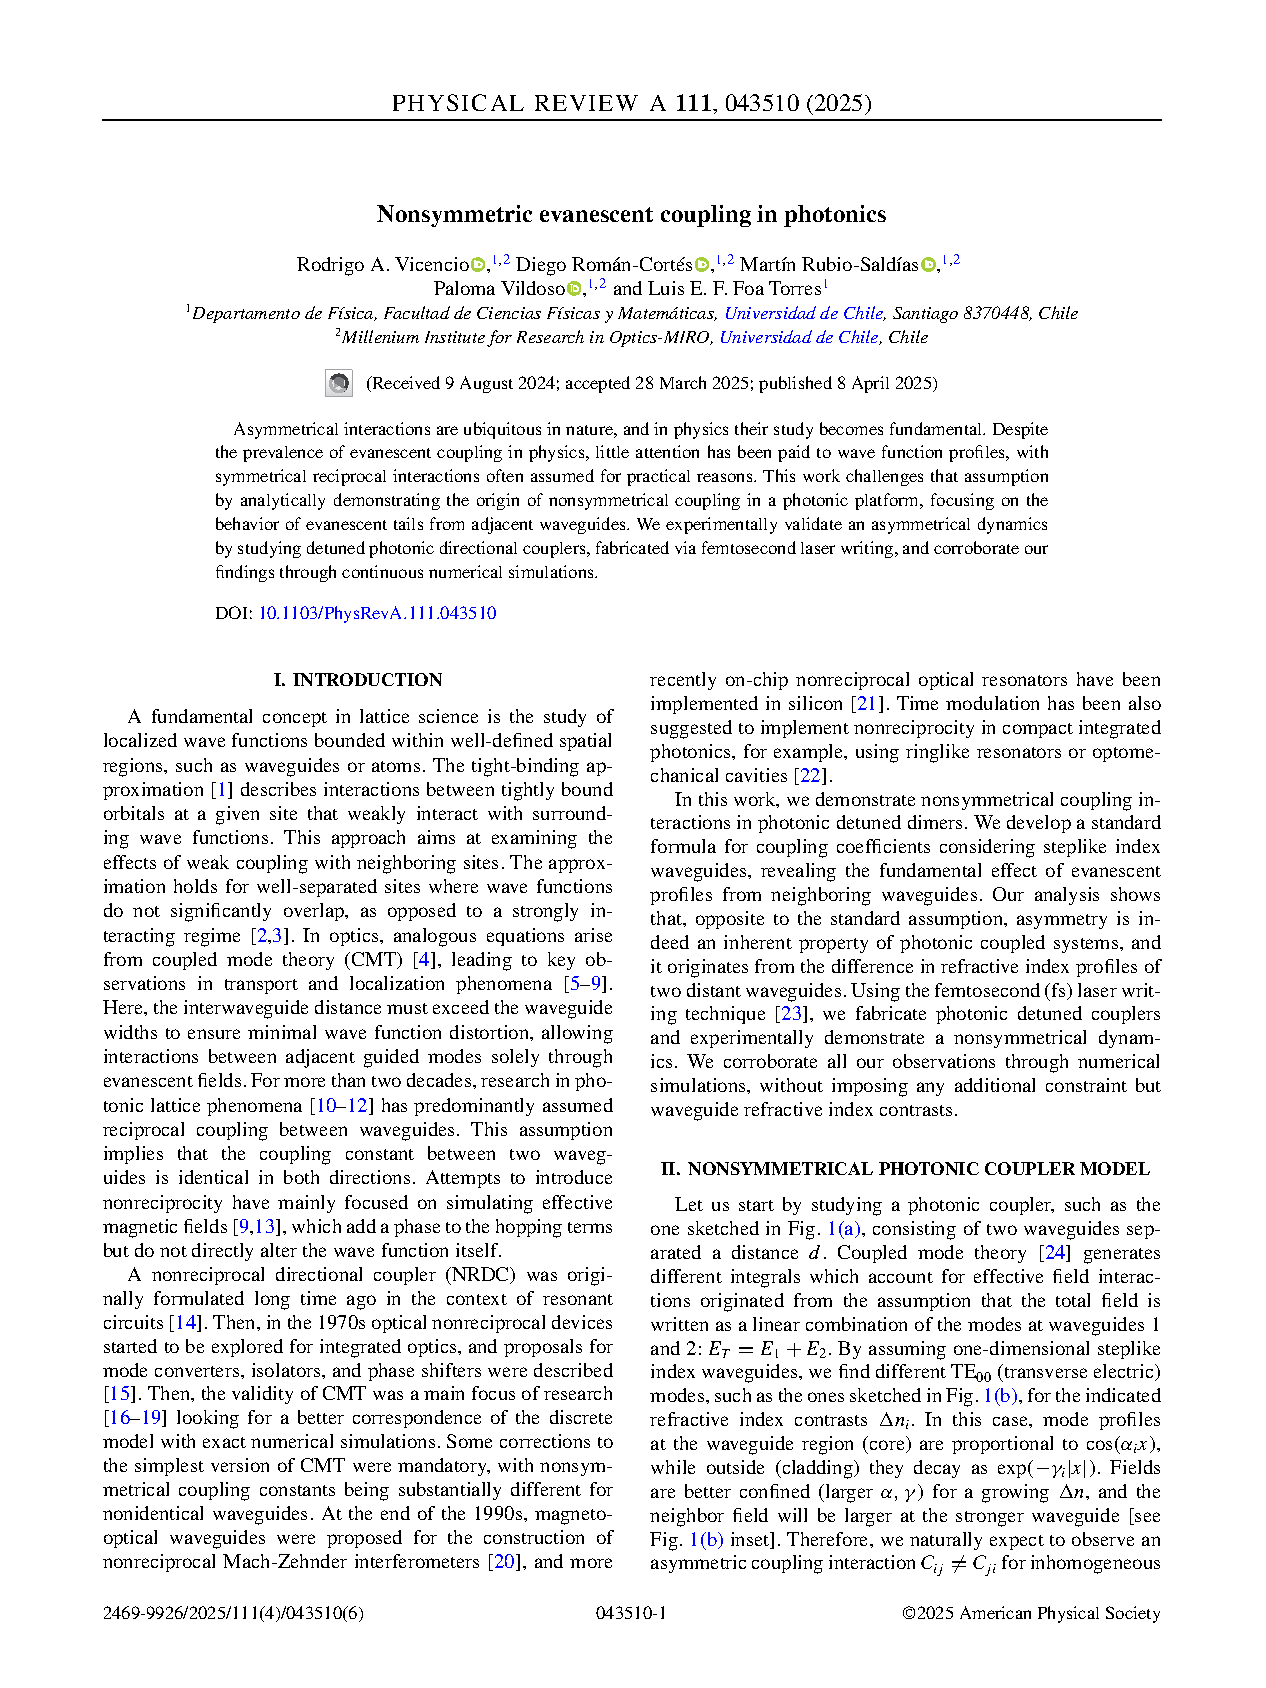
\includegraphics[page=1, width=\linewidth]{media/nonsympap.pdf}
\end{figure}
\newpage
En proceso de referato de la revista \textit{Physical Review Letters}:
\begin{figure}[H]
	\centering
	\includegraphics[page=1, width=\linewidth]{media/2Dradpap.pdf}
\end{figure}